\documentclass{article}
% \usepackage[left = 1cm, top = 1cm, bottom = 1cm, right = 1cm]{geometry}
\usepackage[margin=1in]{geometry}

\usepackage[T1]{fontenc}
\usepackage[fontsize=10pt]{fontsize}

\usepackage{fancyhdr}
\usepackage{extramarks}
\usepackage{amsmath}
\usepackage{amsthm}
\usepackage{amsfonts}
\usepackage{tikz}
\usepackage[plain]{algorithm}
\usepackage{algpseudocode}
\usepackage{multicol}
\usepackage{url}			       
\usepackage{hyperref}
\usepackage{pgf}
\usepackage{xcolor}
\usepackage{minitoc}
\usepackage{bookmark}

\definecolor{umblue}{HTML}{00274C}
\definecolor{ummaize}{HTML}{FFCB05}
\usetikzlibrary{automata,positioning}

\linespread{1}

\pagestyle{fancy}
\lhead{\hmwkAuthorName}
\chead{\hmwkClass: \ \paprTitle}
\rhead{\today}
\lfoot{\hmwkTitle}
\cfoot{\thepage}

\renewcommand\headrulewidth{0.25pt}
\renewcommand\footrulewidth{0.25pt}

\setlength\columnseprule{.25pt}
\setlength{\columnsep}{2.5pc}
\setcounter{secnumdepth}{0}

\newcommand{\hmwkTitle}{Final Project Report}
\newcommand{\paprTitle}{\\ Fundamentals of Microprocessor Design}
\newcommand{\hmwkDueDate}{April 27, 2023 @ 18:00, EST}
\newcommand{\hmwkClass}{CSC 565 - Computer System Architecture}
\newcommand{\hmwkAuthorName}{\textbf{Cason Konzer}}


\title{
    \vspace{2in}
    \textmd{\textbf{\hmwkClass:\ \\ \hmwkTitle}}\\
    \normalsize\vspace{0.1in}\small{Due\ on\ \hmwkDueDate}\\
    \vspace{0.1in}\Large{\textit{\paprTitle}}
    \vspace{3in}
}

\author{\hmwkAuthorName}
\date{\today}

\begin{document}

\maketitle

\pagebreak

\tableofcontents
\listoftables
\listoffigures

\newpage

\section{Introduction}

\subsection{Requirements}
Within the final project for \textbf{CSC 565} I was tasked with creating a simple microprocessor on 8 bit registers. 
This microprocessor was to follow the following specifications:
\begin{itemize}
    \item[\(\diamond\)] Inputs (data and instructions) are received from outside the processor, computed flags and results are to be stored in a register.
    \item[\(\diamond\)] The processor takes all operands directly from internal registers.
    \subitem \(\ast\) operands are not to be passed to the ALU from the instruction itself.  
    \item[\(\diamond\)] The processor must support integer subtraction and logical or as operations. 
    \item[\(\diamond\)] The processor must support sign and overflow flags.
    \subitem \(\ast\) flags are internal and must not be output. 
    \item[\(\diamond\)] The destination for all instructions should first be an internal register, and in the (next) clock cycle following the instruction load the computed output should be sent on the output bus.
\end{itemize}

\noindent
A series of deliverables were specified to guide students in the project in the following manner:
\begin{enumerate}
    \item Draft \& finalized specifications document containing:
    \subitem \(\circ\) Block diagram with input/output pins.
    \subitem \(\circ\) Number of registers and their sizes.
    \subitem \(\circ\) Instruction set with defined operands.
    \subitem \(\circ\) Definition of clock signal.
    \subitem \(\circ\) Timing diagram for example instructions.
    \item Designed device to the specs in Verilog.
    \item Tested and properly functioning device.
    \item Final project report.
\end{enumerate}

\subsection{Motivation}
From the basic specifications and deliverables outlines above I had a solid scope of what was required of me, competencies I had, and competencies I needed to gain. 
In general this project was self guided and required a proactive student to succeed. 
For myself, I got an early start and had been following the corse ahead of schedule, thus this was well catered. 
What I found extremely motivating was the process itself, and getting hands on with the logic of hardware. 
Working with microprocessor devices, in an environment where they are designed all the way from the hardware and software, to the actual integration, gaining a solid understanding of the lower level workings was critical to me. 
With the foundation laid, I will now walk my way through each of the deliverables reflecting on progress made, challenges faces, individual learnings, and potential pitfalls. 

\section{Fundamentals}
\subsection{Where I Stood}
Clear from the outset was that I was an incompetent microprocessor designer, and I had much to learn. 
Many times I have seen colleagues working on wiring diagrams but never myself. 
My first task at hand was to build a fundamental understanding of the concepts which would be utilized. 
I started off by identifying my competencies that were built upon prior readings, class lectures, and assignments. 
Concepts which were understood included:
\begin{itemize}
    \item[\(\diamond\)] What Registers are.
    \item[\(\diamond\)] How block diagrams generally looked.
    \item[\(\diamond\)] Basics of instructions.
    \item[\(\diamond\)] Flags and what they represent.
    \item[\(\diamond\)] The stepping form factor of a clock signal.
\end{itemize}

\noindent
Unclear to me was: 
\begin{itemize}
    \item[\(\diamond\)] Register functional design.
    \item[\(\diamond\)] Clock Location.
    \item[\(\diamond\)] Clock signal generation.
    \item[\(\diamond\)] Synchronization via clocks.
    \item[\(\diamond\)] Instruction set encoding.
    \item[\(\diamond\)] Overflow flag computation.
    \item[\(\diamond\)] Timing diagrams.
    \item[\(\diamond\)] Verilog programming.
\end{itemize}

\subsection{Information Retrieval}
My initial investigations started with a brief overview of the sign, carry, and overflow flag, followed by more detailed views of their operations \cite{stack_binof, ebsmadl_ofs, stack_carry, wiki_negflag, wiki_ovfflag}.
Feeling now more confident in flags I proceeded to dig into registers and how they function \cite{neso_diff, neso_srlatch, neso_triggering}.
At this point I was still fuzzy on clocks and thus I did some reading up on them as well \cite{stack_ieclk, neso_clk, stack_oscii, wiki_clock}.
Before programming in Verilog I needed a more sound knowledge of combinatorial logic and thus proceeded to get an understanding of what lay inside the blocks which I would be placing in my pinouts \cite{et_binadd, et_binsub, et_combilog, et_digtcomp, et_demultiplex, et_multiplex, icacuk}.
In order to implement my logic in Verilog I would needed to know how to program in it \cite{coursera_fpga, rtd_fpga}. 
Last for testing my machine I would need to utilize a scripting language. 
Most familiar to me is Python, but for bit manipulation in the language I required background \cite{geeks_twos, stack_twos, pywiki_bit, stack_logitwos, geeks_ones}. 
Despite the plethora of cited materia this does not encompass everything and thus is incomplete. 
The foundation is also well complemented by the professor's (Dr. Zahid Syed's) teachings and the class textbooks \cite{Bryant, Hennessy}. 

It is with this foundation that I learned the fundamentals of combinatorial logic, flag computation, and register operation. 
The sign flag I found quite trivial, but an analysis on inputs and outputs provided an elegant way of testing for overflow I was happy to see. 
I learned about latches and flip flops in registers, which greatly helped me understand the lockstep nature of microprocessors. 
With this under my belt I was able to start dabbling in Verilog using tools provided by Xilinix and Aldec. 
I started creating block diagrams and synthesizing them into code to get a feel for the language. 
I would first draw them out and then port them into the programming environment. 
I took the sample code from the professor and modified it to similar use cases. 
I learned the pros and cons of internal and external clocks, and how to read timing diagrams. 
At this point I was ready to start specifications while designing in the background. 

\section{Microprocessor Specifications \& Design}
\subsection{Bottom Up Approach}
Generally speaking, specifications and design were paired tasks. 
It was specifications which drove initial design, but it was realizations of issues and optimizations in the design which granted revisions to the specifications. 
The process started with defining the registers, which enabled me to visualize the first linking of the operand registers to the ALU. 
Form this point it was crucial for me to analyze the inputs and outputs. 
How the processor knew data was valid and where to send it was realized by enabling pins and a input data bus. 
For myself, it was fundamental to work first on a bit level rather than a byte level. 
My initial diagrams contained 8 separate input wires rather than one input bundle for the data bus. 
I next made a definitive choice to use an external clock, while in practice I would prefer support for both internal and external clocks, this simplified the design. 

I next started to define the instruction set, and its encoding. 
From here I was able to link the ALU to the instruction register. 
While at first my block diagram was criticized for being too granular, the bottom up approach I took gave me depth in understanding the microprocessor. 
This made it extremely easy to generalize my design and block diagram to a more abstract level. 
Initially I thought that I would have the ALU output the computed results to a designated register, and the flags to a dedicated register as well. 
Upon further revision I realized that my instruction set needed not all of the bits packed into a byte to encode all possible instructions. 
Additionally, I realized that given a 2 bit enable input I need not even provide load instructions, but this could rather be encoded into the enable bits. 
As a result I decided to pack the ALU flags into the already determined instruction register and further simplify the design. 
In a similar manner, I realized that I need not an ALU output register, but I could instead write back to the operand registers. 

\subsection{Handling Pitfalls}
What occurred as a result was a race condition such that as operand register values were updated, if the instruction register was not flushed, the ALU would continuously perform the instruction on the new register values. 
In order to mitigate this issue I needed to encode an operation flag into the instruction register which would update with the clock. 
I decided to leverage an already defined portion of the instruction encoding, the destination encoding. 
The destitution encoding defined where the ALU was to write back to, being the data bus, and one or both of the operand registers. 
My solution was to update the instruction register with the destinations encoding `00' which specified only output bus writing, thus mitigating the race condition. 
This process was done every clock cycle but only if the enable pins had been set to disable instruction loads. 
In the case that the enable pins were set to load data, regardless of the location, the writing of the ALU to any location was by default disabled. 
In the end I had created a microprocessor designed to operate in an embedded real-time manner. 
The hardware requirements were absolutely minimized, as well as the required intermediate buffering registers. 
The specifications for such a system are realized in the Appendices.

\section{Microprocessor Testing}
\subsection{The Test Bench}
In testing such a system I started with an iterative approach.
I used the professors base code to create simple test vectors, at first by hand. 
This was sufficient for 2 and 4 bit operands, but became increasingly complex for 8 bit operands, or multiple inputs. 
Everything at first was designed on the bit level and I soon realized that this made not only my Verilog code overly complex, but also the requirements for testing my models. 
I was writing then my test vectors though Python, and importing the files into ActiveHDL. 
I decided at this point it would be beneficial to refactor my code, and in doing so I found a nice repository which extended some of my previous bitwise functions for multiplexing and addition to bytewise \footnote{\url{https://github.com/neelkshah/MIPS-Processor}}.
This made my test cases much simpler to write, but still I needed to formulate a mathematical model in a higher level language for comparison. 
Leveraging the bit manipulation skills I learned in Python I created such models and evolved my test benches to self checking test benches. 
I randomized operand inputs and extensively tested each instruction to ensure proper functionality. 
In the end my processor functioned as expected without issue. 

\subsection{Design Changes}
As mentioned above the switch to writing Verilog on bundles of wires (or vectors), rather than individual wires (bits) was a design change driven by my testing. 
Additionally Testing and analysis of waveforms gave me the realization that within my code there were still some buffer register for the operands when feeding into the ALU. 
In part this was a countermeasure to at first deal with the race condition, but more generally this was a realization that still I had not a great grasp on programming in Verilog. 
I continued to explore external resources while taking a Coursera course on the material which gave me a much deeper understanding of the logic Verilog was implementing, tools it had available, and a secondary VHDL perspective. 
Knowing then the differences between asynchronous and synchronous operations, I again refactored my code to eliminate the temporary registers. 
In this manner I separated out much of the combinatorial logic into their own modules, which I then linked to the controlling logic. 
After a final revision I was happy with my design and the timing diagrams it produced, the before and after are shown in Figure~\ref{fig:bad_timing} and Figure~\ref{fig:good_timing}.
In a similar manner evolution of the design can be seen through the microprocessor's block diagrams Figures~[\ref{fig:block0},\ref{fig:block1},\ref{fig:block2},\ref{fig:block3},\ref{fig:block4}]. 
The microprocessor was minimal and functional, only the necessary components were used. 

\section{Summary}
In summary I learned a plethora about how microprocessors actually work, and how the design process takes place. 
Not only the technical skills did I manage to gain, but additionally communication, documentation, and planning skills. 
This project taught me how to keep a well established communication channel with my peers, although my group did eventually dissolve. 
I managed scheduling meetings with my peers and educating them on the background topics I learned. 
I took the opportunities to learn from them, and converse on course topics, which helped me to identify my knowledge gaps.  
I assigned tasks collaboratively and followed up with the members, although most often they had not held up their end of the bargain. 
I was fast to communicate concerns not only directly to my peers, but also to the professor of the unfolding situation. 
In doing so I found myself necessarily working ahead and completing the tasks assigned to peers. 
As two of the students ended up dropping the class, I prevented myself from being in a scramble at the end of the semester. 
To me, being ahead of the game was necessary, as I never knew when there might be a sudden spike in my day to day employments. 

Drawing out the block diagrams, and writing up truth tables proved to be one of my most useful tools. 
By doing so I was forced to visualize and compute the architecture and modules myself. 
This process greatly deepened my understanding and allowed me to fluently explain, and show the concepts to group members. 
Documentation for my background resources was shared and recommended, alternative resources were sought for struggles applying specifically to the peers and not myself. 
In citing my references I realized the importance of even more extensive documentation, as there were many valuable resources I found to be `common knowledge' which in any case are due credit. 
I learned how to program in Verilog, and design a system from the bottom up, test it and verify it's functionality. 
This has been by far my favorite class, and the project was a pleasure. 
I am grateful that I can now have more technical conversations on computing architecture, and speak from this experience. 

\newpage

\section{Appendix : Tables}

\begin{table}[h!]
    \centering
    \begin{tabular}{|c||c|} 
        \hline
        Register & Description \\
        \hline
        \hline
        IR & Instruction Register + Flags \\
        \hline
        R0 & Operand Register 0 \\
        \hline
        R1 & Operand Register 1 \\
        \hline
    \end{tabular}
    \caption{Register Specifications.}
    \label{tab:regs}
\end{table}

\begin{table}[h!]
    \centering
    \begin{tabular}{|p{0.09\linewidth}||p{0.075\linewidth}|p{0.06\linewidth}|p{0.0775\linewidth}|p{0.0775\linewidth}|p{0.085\linewidth}|p{0.085\linewidth}|p{0.1\linewidth}|p{0.1\linewidth}|} 
        \hline
        Bit & 7 & 6 & 5 & 4 & 3 & 2 & 1 & 0 \\
        \hline
        \hline
        Encoding & Overflow Flag & Sign Flag & OR \ \ \ OpCode & SUB OpCode & Operand 1 & Operand 0 & Destination 1 & Destination 0 \\
        \hline
    \end{tabular}
    \caption{IR Encoding.}
    \label{tab:irenc}
\end{table}

\begin{table}[h!]
    \centering
    \begin{tabular}{|c|c||c|} 
        \hline
        IR Bit 1 & IR Bit 0 & Write Back Location \\
        \hline
        \hline
        0 & 0 & Bus \\
        \hline
        0 & 1 & R0 \& Bus \\
        \hline
        1 & 0 & R1 \& Bus \\
        \hline
        1 & 1 & R0 \& R1 \& Bus \\
        \hline
    \end{tabular}
    \caption{Destination Encoding.}
    \label{tab:destenc}
\end{table}

\begin{table}[h!]
    \centering
    \begin{tabular}{|c|c||c|} 
        \hline
        IR Bit 5 & IR Bit 4 & Operands \\
        \hline
        \hline
        0 & 0 & R0, R0 \\
        \hline
        0 & 1 & R1, R0 \\
        \hline
        1 & 0 & R0, R1 \\
        \hline
        1 & 1 & R1, R1 \\
        \hline
    \end{tabular}
    \caption{Operand Encoding.}
    \label{tab:openc}
\end{table}

\begin{table}[h!]
    \centering
    \begin{tabular}{|c|c||c|} 
        \hline
        IR Bit 5 & IR Bit 4 & ALU Operation \\
        \hline
        \hline
        0 & 0 & No-Op \\
        \hline
        0 & 1 & SUB \\
        \hline
        1 & 0 & OR \\
        \hline
        1 & 1 & No-Op \\
        \hline
    \end{tabular}
    \caption{Operation Encoding.}
    \label{tab:optenc}
\end{table}

\newpage

\section{Appendix : Figures}

\begin{figure}[ht!]
    \centering
    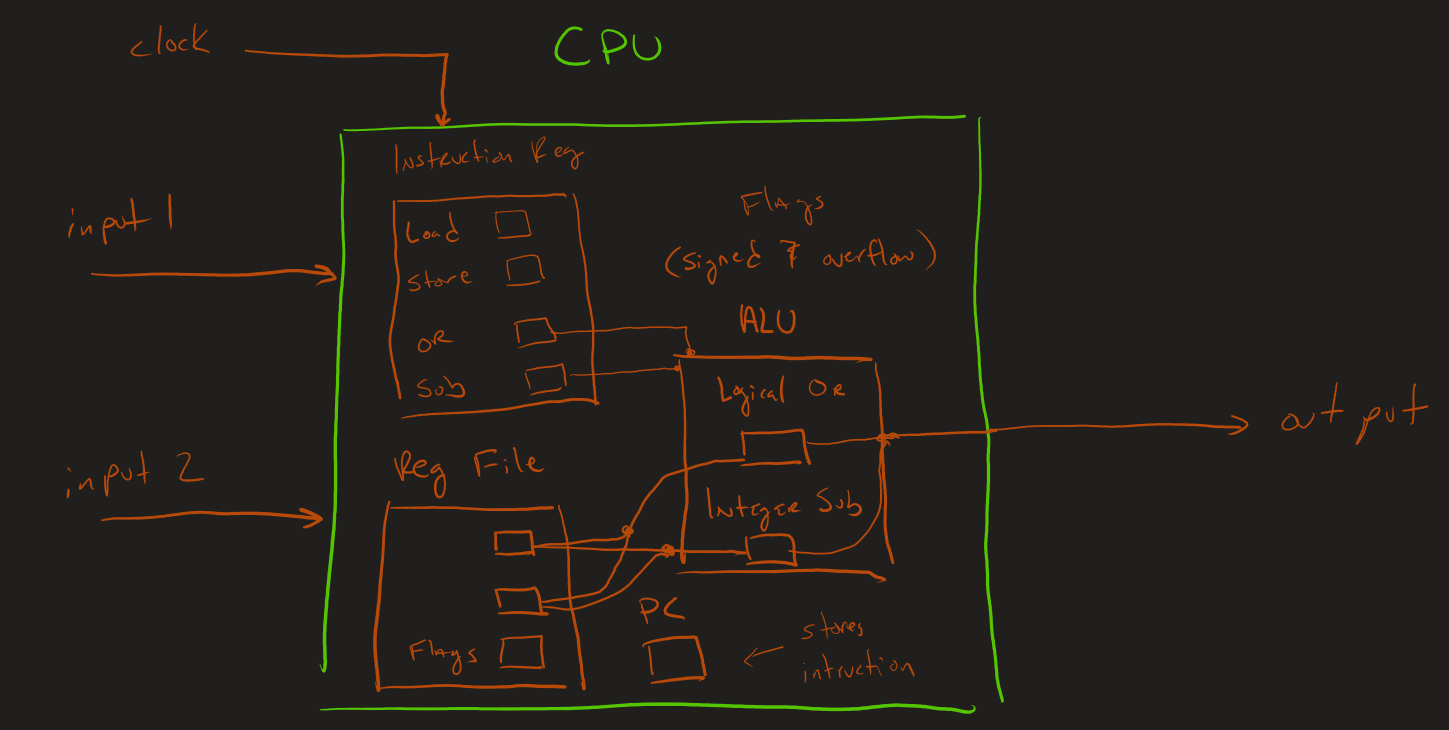
\includegraphics[width=\textwidth]{./_img/Block_Diagram_v0.PNG}
    \caption{Initial Microprocessor Block Diagram.}
    \label{fig:block0}
\end{figure}

\begin{figure}[ht!]
    \centering
    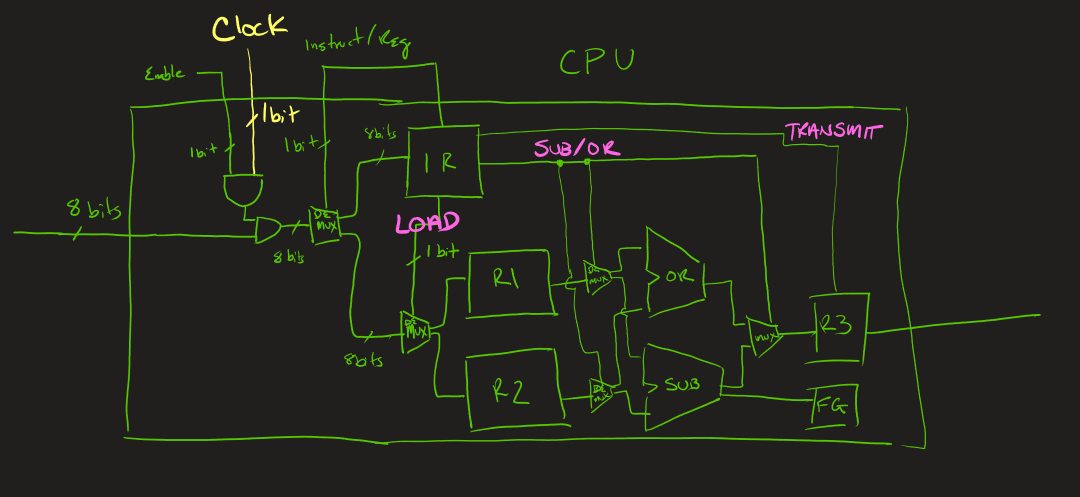
\includegraphics[width=\textwidth]{./_img/Block_Diagram_v1.PNG}
    \caption{First Revised Microprocessor Block Diagram.}
    \label{fig:block1}
\end{figure}

\pagebreak

\begin{figure}[ht!]
    \centering
    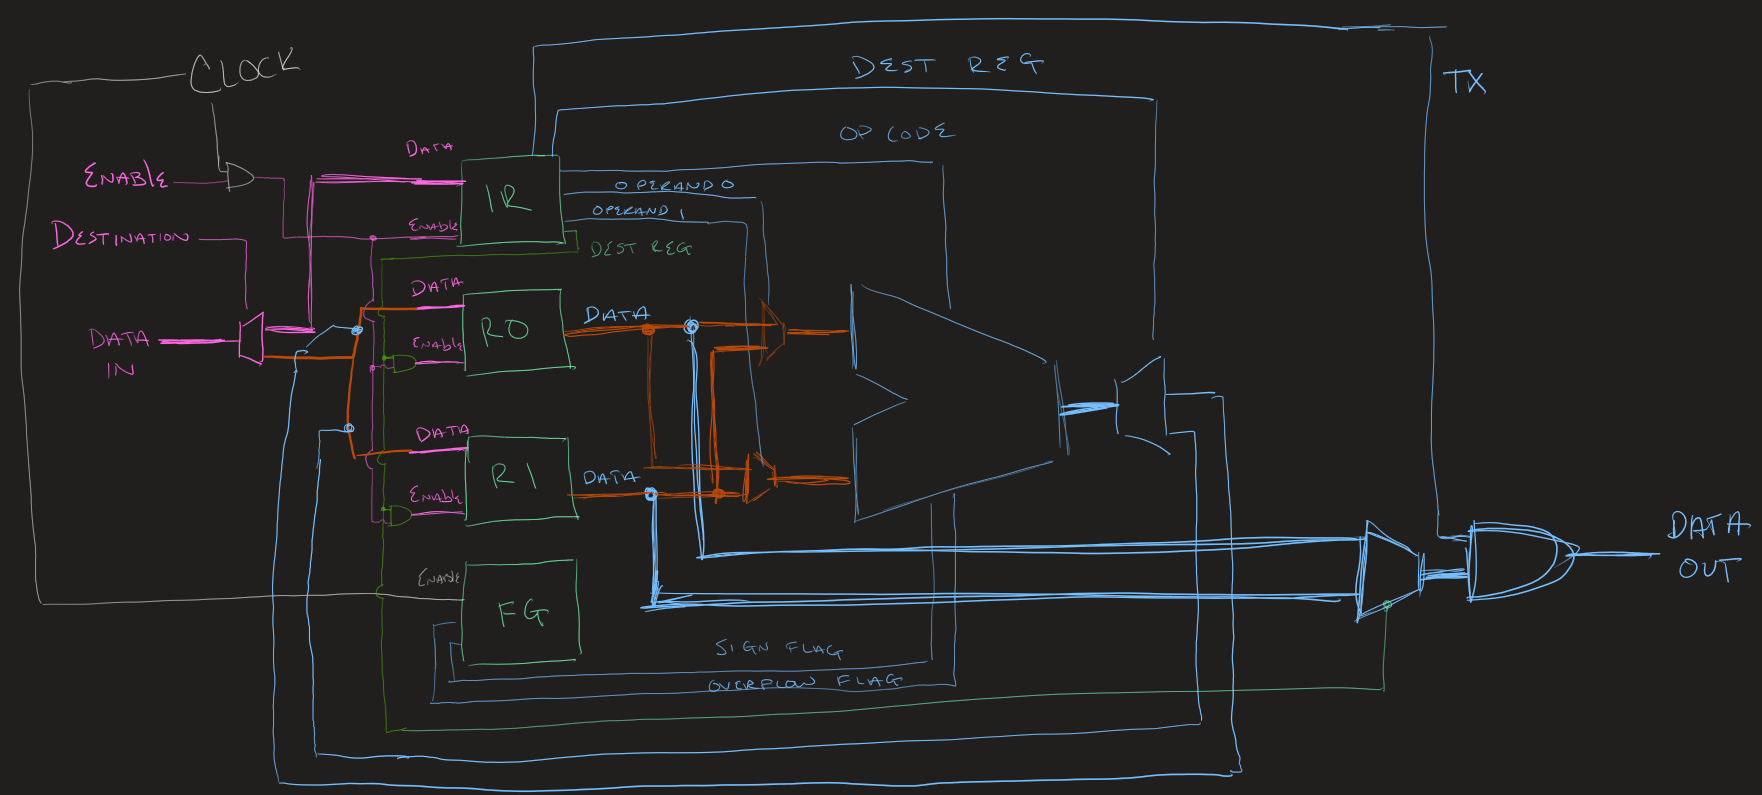
\includegraphics[width=\textwidth]{./_img/Block_Diagram_v2.PNG}
    \caption{Second Revised Microprocessor Block Diagram.}
    \label{fig:block2}
\end{figure}

\begin{figure}[ht!]
    \centering
    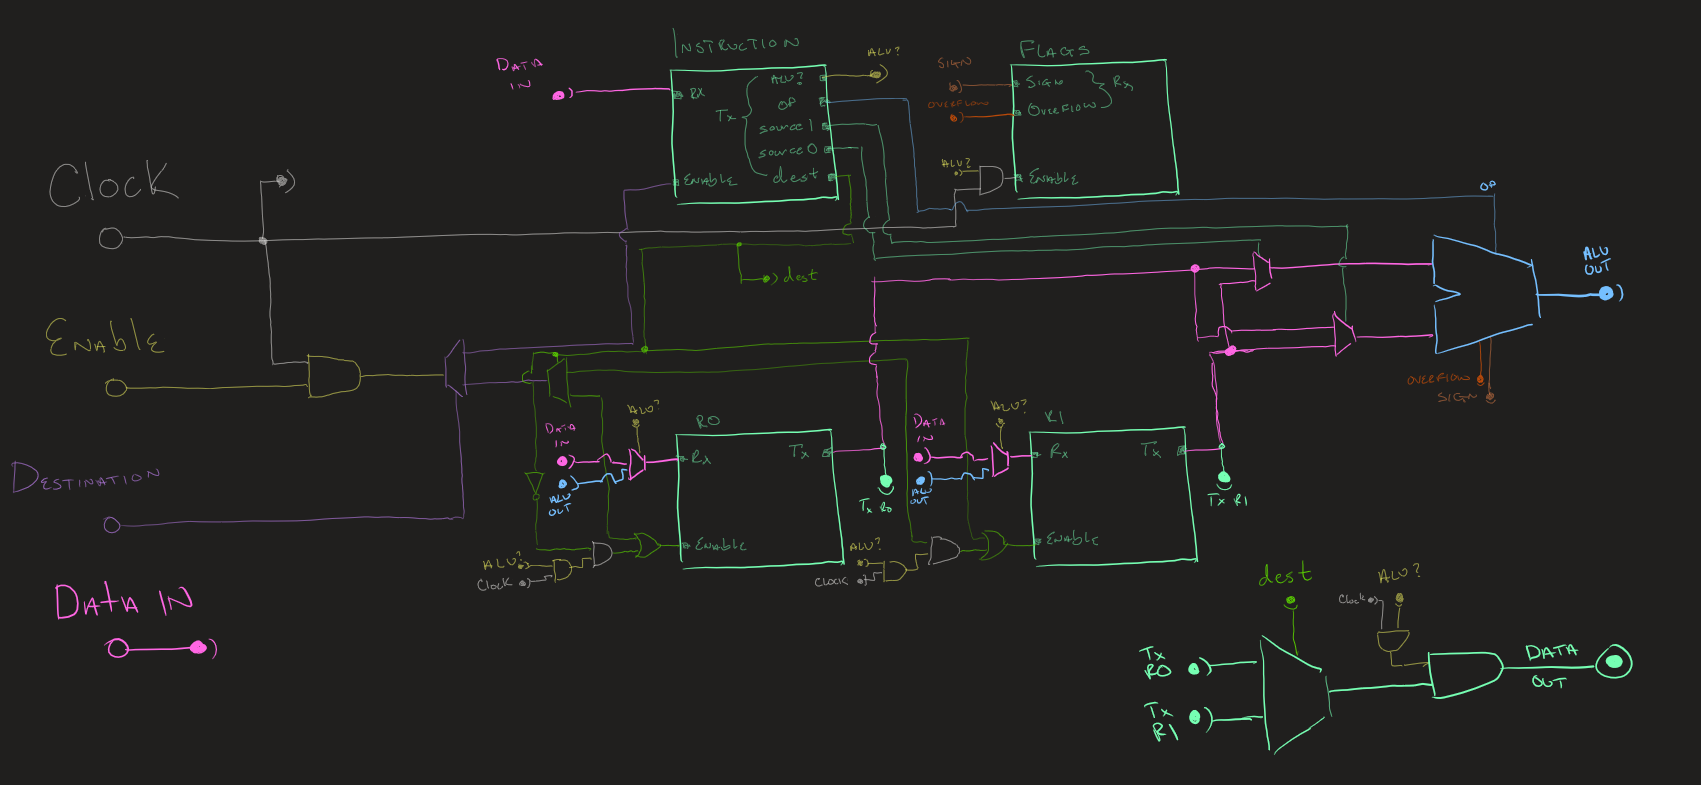
\includegraphics[width=\textwidth]{./_img/Block_Diagram_v3.PNG}
    \caption{Third Revised Microprocessor Block Diagram.}
    \label{fig:block3}
\end{figure}

\pagebreak

\begin{figure}[ht!]
    \centering
    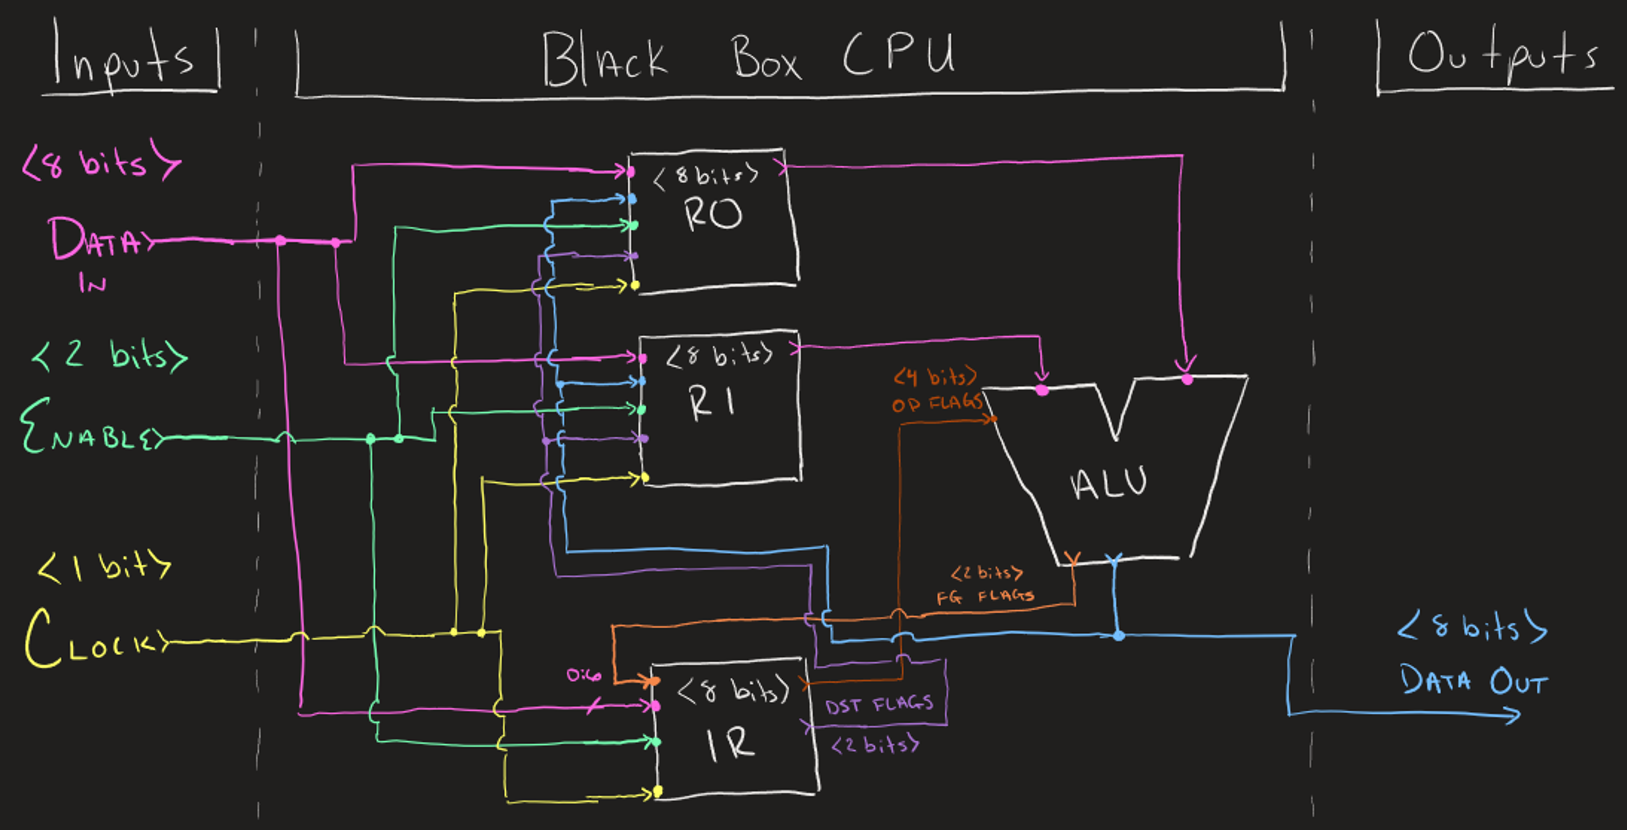
\includegraphics[width=\textwidth]{./_img/Block_Diagram.PNG}
    \caption{Final Microprocessor Block Diagram.}
    \label{fig:block4}
\end{figure}

\begin{figure}[ht!]
    \centering
    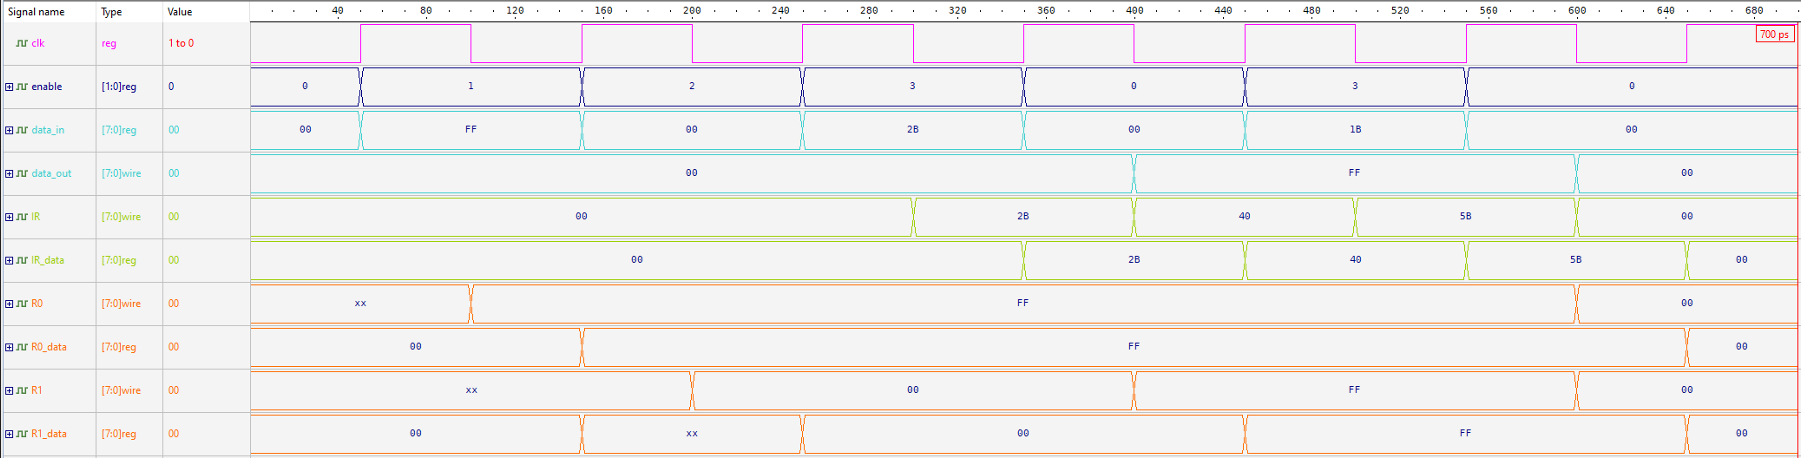
\includegraphics[width=\textwidth]{./_img/Bad_Timing.PNG}
    \caption{Initial Timing, with buffer registers.}
    \label{fig:bad_timing}
\end{figure}

\begin{figure}[ht!]
    \centering
    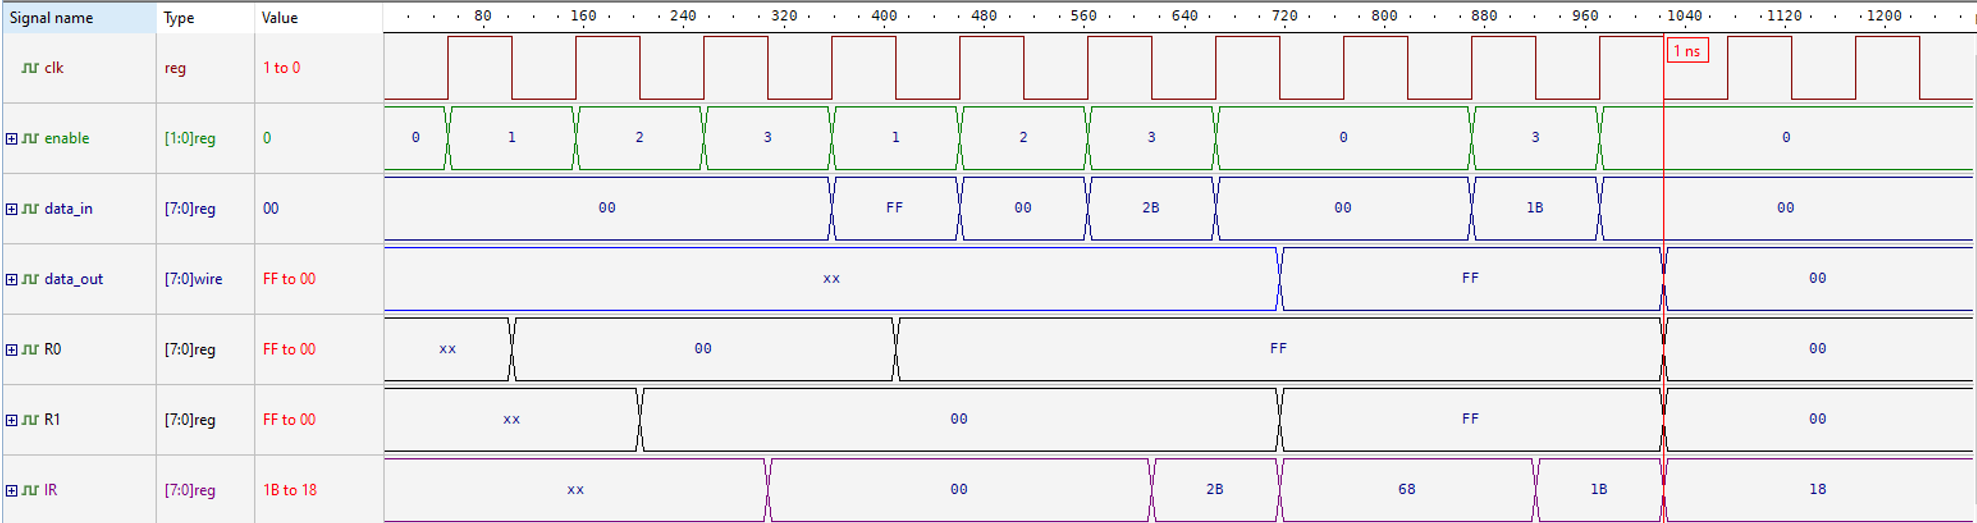
\includegraphics[width=\textwidth]{./_img/Good_Timing.PNG}
    \caption{Revised Timing, with inserted no-ops.}
    \label{fig:good_timing}
\end{figure}

\pagebreak
\newpage

\bibliographystyle{acm} % abbrv, acm, alpha, apalike, ieeetr, plain, siam, unsrt, tugboat, plainurl
\bibliography{./konzer_cason_csc_565_final_project_report.bib}{}
\end{document}